
\documentclass[conference]{IEEEtran}
\IEEEoverridecommandlockouts

\usepackage{cite}
\usepackage{amsmath,amssymb,amsfonts}
\usepackage{algorithmic}
\usepackage{graphicx}
\usepackage{textcomp}
\usepackage{xcolor}
\usepackage{booktabs}
\usepackage{array}
\usepackage[linesnumbered,ruled,vlined]{algorithm2e}

\def\BibTeX{{\rm B\kern-.05em{\sc i\kern-.025em b}\kern-.08em
    T\kern-.1667em\lower.7ex\hbox{E}\kern-.125emX}}

\begin{document}

\title{Grid-Based Vehicle Maneuver Prediction at Road Intersections Towards Proactive V2N Handover in 5G/B5G Networks}

\author{
\IEEEauthorblockN{1\textsuperscript{st} Heriansyah}
\IEEEauthorblockA{\textit{Institute of Telecooperation} \\
\textit{Johannes Kepler University Linz}\\
Linz, Austria \\
k12121057@students.jku.at}
\and
\IEEEauthorblockN{2\textsuperscript{nd} Gabriele Kotsis}
\IEEEauthorblockA{\textit{Institute of Telecooperation} \\
\textit{Johannes Kepler University Linz}\\
Linz, Austria \\
gabriele.kotsis@jku.at}
}

\maketitle

\begin{abstract}
Proactive handover management in Vehicle-to-Network (V2N) communications over 5G requires accurate prediction of vehicle trajectory, especially at road intersections where a vehicle may proceed in multiple directions, each served by a different gNodeB cell.
This paper proposes a behavior-fused, grid-based vehicle maneuver prediction framework as a foundational component for such proactive handover systems.
The method combines lane-conditional transition probability databases with two lightweight behavioral cues extracted from recent trajectory observations: a deceleration ratio and a lateral drift measure.
A per-lane probabilistic database is constructed from training trajectories on a 10\,m grid, and at inference time, behavioral bias weights are fused with the database prior through a linear interpolation scheme to predict the maneuver class (left, straight, or right) at the intersection.
The framework is topology-agnostic and is validated on synthetic datasets covering four-way, T-junction, and Y-junction intersection types.
Results demonstrate that behavioral cue fusion substantially improves maneuver classification accuracy over database-only and Markov-based baselines, while maintaining low computational complexity suitable for real-time embedded deployment.
\end{abstract}

\begin{IEEEkeywords}
maneuver prediction, intersection, grid-based model, behavioral cues, autonomous driving, trajectory prediction
\end{IEEEkeywords}

% =========================================================================
\section{Introduction}
\label{sec:intro}

The deployment of 5G networks has enabled new Vehicle-to-Network (V2N) capabilities by supporting high data rates and low-latency communication between vehicles and cellular infrastructure \cite{pawar2024intelligent}.
As vehicles move through the network coverage area, they must continuously maintain connectivity by performing handover from one gNodeB cell to another.
In high-mobility vehicular scenarios, rapid signal fluctuations and outdated measurement reports make traditional reactive handover unreliable, causing handover failures, ping-pong effects (back-and-forth handovers), and unnecessary handovers, which negatively impact network reliability as well as Quality of Service (QoS) and Quality of Experience (QoE) for end-users \cite{sun2021multi}.

Proactive handover addresses this issue by predicting the vehicle’s future position and selecting the optimal target gNodeB before signal degradation occurs. 
On straight road segments, trajectory prediction is relatively simple because the vehicle is likely to remain on the same road, and a one-step Markov model is often sufficient. 
The main challenge arises at road intersections, where a vehicle may turn left, continue straight, or turn right, with each path leading toward a different gNodeB coverage cell. 
Without knowing the intended maneuver, the network cannot determine which gNodeB should be prepared for handover, which may result in premature attachment to the wrong gNodeB and inefficient use of radio resources.

Existing maneuver prediction methods that rely only on instantaneous heading or speed often yield unstable classifications near the intersection decision point, where small measurement noise can trigger large prediction swings \cite{katrakazas2015real}. 
Data-driven deep learning approaches \cite{altche2017lstm, lefkopoulos2021interaction} can improve accuracy, but they typically require GPU hardware, large annotated datasets, and online training, which is poorly suited to the real-time, resource-limited constraints of embedded V2N units. 
In 5G connected vehicles, the onboard compute unit must also handle radio resource management, sensor fusion, and real-time communications, leaving little headroom for computationally intensive inference. 
A lightweight prediction algorithm that runs on a low-power embedded processor, without expensive matrix operations or neural network inference, is therefore essential for practical V2N deployment.

To bridge the gap between prediction accuracy and computational constraints, this paper proposes a behavior fused, grid based maneuver prediction framework as a foundational module for proactive V2N handover in 5G/B5G networks. 
The proposed framework combines a lane conditional probabilistic database with two lightweight behavioral cues, deceleration ratio and lateral drift, to predict the intended maneuver at road intersections as left, straight, or right, without requiring deep learning.

The main contributions of this paper are as follows:
\begin{itemize}
  \item We propose a dynamic fusion mechanism that significantly improves the accuracy of standard grid-based transition priors by analytically incorporating the vehicle's real-time behavioral context, specifically deceleration and lateral drift.
  \item We design a fully topology-agnostic method that can be applied to diverse intersection geometries (e.g., four-way, T-junction, Y-junction) out-of-the-box without requiring intersection-specific retraining or structural changes.
  \item We develop a framework that resolves critical maneuver ambiguities (such as distinguishing straight-ahead motion from impending turns) using strictly lightweight arithmetic operations, thereby meeting the stringent computational constraints of embedded V2N systems.
\end{itemize}

The remainder of this paper is organized as follows.
Section~\ref{sec:related} reviews related work.
Section~\ref{sec:method} describes the proposed method and experimental setup.
Section~\ref{sec:experiments} presents results.
Section~\ref{sec:conclusion} concludes the paper.

% =========================================================================
\section{Related Work}
\label{sec:related}

Maneuver prediction at road intersections is a long-studied problem in autonomous driving and intelligent transportation research.
Early approaches rely on physics-based motion models such as constant-velocity or constant-turn-rate dynamics, extended by Interacting Multiple Model (IMM) filters to handle discrete mode switching \cite{lefevre2014survey}.
These methods are computationally efficient and require no training data, but they assume a limited set of motion primitives and lack the geometric awareness needed to reliably distinguish between multiple exit directions at complex junctions.

As data availability grows, machine learning approaches emerge as more expressive alternatives.
Methods based on support vector machines \cite{schmerling2018multimodal}, recurrent neural networks \cite{altche2017lstm}, and graph neural networks \cite{lefkopoulos2021interaction} substantially improve prediction accuracy by learning context-dependent motion patterns from large annotated datasets.
Despite their effectiveness, these models require significant computational resources at inference time, rely on offline training phases, and offer limited transparency to system designers.
For resource-constrained embedded units in 5G-connected vehicles, which must simultaneously manage radio resource allocation, sensor fusion, and real-time communication, the runtime memory and latency demands of deep models are often prohibitive.

Grid-based trajectory models offer a compelling middle ground by discretizing the environment into cells and estimating statistical transition distributions from observed data \cite{katrakazas2015real}.
These models are compact, interpretable, and efficient at query time.
However, a critical limitation of standard grid approaches is the absence of lane conditioning: when vehicles approaching from multiple directions all contribute to the same cell statistics, the resulting distributions become ambiguous and misleading for turn prediction at intersections.

Behavioral cue incorporation represents an important direction for intersection-specific prediction.
Prior work such as \cite{klingelschmitt2014combining} demonstrates that deceleration and lateral displacement signals carry predictive information beyond heading alone.
However, existing methods that exploit such cues typically rely on trained classifiers, requiring labeled datasets and model fitting.
In contrast, the proposed framework fuses two interpretable behavioral scalars---deceleration ratio and lateral drift, analytically into a probabilistic prior, eliminating the need for classifier training while retaining full system transparency.
Compared to all three families of prior work, the proposed approach uniquely combines lane conditioning, behavioral cue fusion, GPU-free inference, and zero offline training, making it well-suited for deployment on embedded V2N units.

% =========================================================================
\section{Proposed Method}\label{sec:method}

This section describes the proposed behavior-fused, grid-based maneuver prediction framework.
The core idea is to build a compact lane-conditional probability database from observed vehicle trajectories, then augment it at query time with two lightweight behavioral cues extracted from recent motion, deceleration ratio and lateral drift.
Together, these components enable the system to disambiguate maneuver intent (left, straight, or right) at road intersections without requiring deep learning or any online training.

\subsection{Grid Discretization}
The continuous 2-D map is discretized into a regular grid with cell size $G = 10$\,m.
A vehicle position $(x, y)$ maps to grid cell indices:
\begin{equation}
  g_x = \lfloor x/G \rfloor + 1, \quad g_y = \lfloor y/G \rfloor + 1.
\end{equation}
Each cell is addressed by a unique integer identifier:
\begin{equation}
  \mathrm{gid} = (g_y - 1) \times 2000 + (g_x - 1).
\end{equation}

\subsection{Lane Classification}
The instantaneous compass heading $\theta$ (degrees, 0 = north, 90 = east) is computed from recent cell-to-cell displacements.
Vehicles are assigned to one of four lanes based on their primary travel direction:
\begin{equation}
  \mathrm{lane} =
  \begin{cases}
    1 & \theta \in [315^\circ, 360^\circ) \cup [0^\circ, 45^\circ) \quad\text{(northbound)} \\
    2 & \theta \in [45^\circ, 135^\circ) \quad\text{(eastbound)} \\
    3 & \theta \in [135^\circ, 225^\circ) \quad\text{(southbound)} \\
    4 & \theta \in [225^\circ, 315^\circ) \quad\text{(westbound)}
  \end{cases}
\end{equation}
This lane assignment ensures that vehicles approaching an intersection from different directions maintain separate probability statistics, preventing cross-directional contamination of the database.
Fig.~\ref{fig:gridlane} illustrates the four-lane partition and the 9-direction probability structure associated with each grid cell.

\begin{figure}[!t]
\centerline{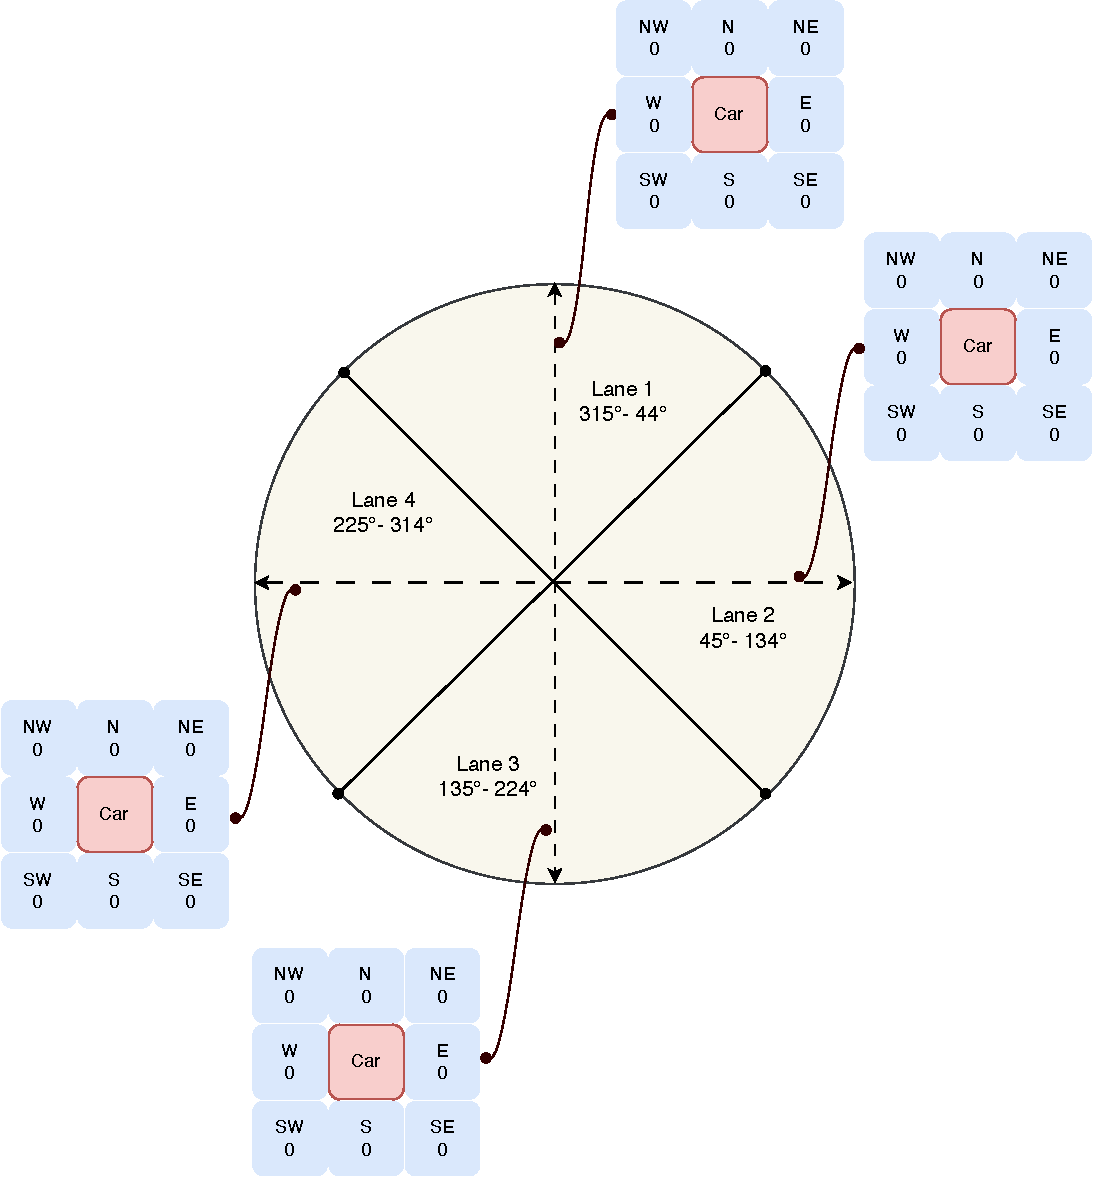
\includegraphics[width=0.95\columnwidth]{img/gridandLane.pdf}}
\caption{Lane classification scheme and grid cell probability structure.}
\label{fig:gridlane}
\end{figure}

\subsection{Lane-Conditional Probability Database}
\label{subsec:db}

During training, each cell-to-cell transition in a trajectory is accumulated as a count $c(d \mid \mathrm{gid}, \mathrm{lane})$, where $d \in \{1,\ldots,9\}$ denotes one of eight compass directions or a stationary state.
Training trajectories are processed in a single pass over the dataset.

At the intersection cell, observations naturally yield counts for left, straight, and right exits.
For cells on straight road segments with a sufficiently dominant direction (empirically, dominant direction probability $\geq 0.85$ and second-highest $< 0.15$), the probability vector is sharpened to a one-hot encoding to reduce noise.
Intersection cells are identified by a second-highest direction probability exceeding a threshold (default 0.12) and are stored with their raw normalized counts.

The database $\mathcal{D}$ consists of four CSV files ($\texttt{dbx\_lane1.csv}$ through $\texttt{dbx\_lane4.csv}$), each mapping $\mathrm{gid}$ to a 9-element probability vector $\mathbf{p}_{\mathrm{base}}$ over the eight compass directions and a stationary state, as illustrated in Fig.~\ref{fig:gridlane}.
At query time, the database is loaded into an in-memory hash map keyed by \texttt{int32} grid identifiers for $O(1)$ lookup.

\subsection{Behavioral Cue Extraction}
\label{subsec:cues}

Two motion cues are extracted from a window of $W$ recent positions centered on the current intersection crossing point $\mathbf{c}_0$:

\textbf{Deceleration ratio} measures the relative speed reduction near the intersection:
\begin{equation}
  r_v = \frac{\bar{s}_{\mathrm{center}}}{\max(\bar{s}_{\mathrm{before}},\, \epsilon)},
\end{equation}
where $\bar{s}_{\mathrm{before}}$ is the mean inter-sample displacement 8--1 steps before $\mathbf{c}_0$, and $\bar{s}_{\mathrm{center}}$ is the mean displacement within $\pm 2$ steps around $\mathbf{c}_0$, and $\epsilon = 10^{-6}$ avoids division by zero.
A value $r_v < 1$ indicates slowdown.

\textbf{Lateral drift} measures the net transverse shift of the trajectory relative to the approach heading:
\begin{equation}
  \Delta_{\mathrm{lat}} = \bar{\ell}_{\mathrm{after}} - \bar{\ell}_{\mathrm{before}},
\end{equation}
where $\ell_i = (\mathbf{p}_i - \mathbf{c}_0) \cdot \hat{\mathbf{n}}$ projects each point onto the unit left-normal $\hat{\mathbf{n}}$ of the incoming direction vector.
A positive $\Delta_{\mathrm{lat}}$ indicates a drift toward the left; negative indicates a drift toward the right.

\subsection{Behavioral Bias Weights}
From the cues, scalar weights are computed:
\begin{align}
  w_{\mathrm{slow}}  &= \mathrm{clip}\!\left((1 - r_v)\,g_s,\; 0,\; 0.6\right), \\
  w_{\mathrm{drift}} &= \mathrm{clip}\!\left(\frac{|\Delta_{\mathrm{lat}}|}{d_{\mathrm{ref}}}\,g_d,\; 0,\; 0.6\right),
\end{align}
where $g_s$ is the slow gain, $g_d$ is the drift gain, and $d_{\mathrm{ref}}$ is a reference drift distance (default: lane width $\approx 1.2$\,m).
The clip operator bounds the weights to $[0, 0.6]$ to prevent behavioral cues from completely overriding the database prior.

\subsection{Behavioral Bias Probability Vector}
A ternary behavioral bias $\mathbf{p}_{\mathrm{bias}} \in \mathbb{R}^3$ over $\{$left, straight, right$\}$ is constructed from the weights:
\begin{equation}
  \mathbf{p}_{\mathrm{bias}} = \left[0.5\, w_{\mathrm{slow}},\;\; 1 - w_{\mathrm{slow}},\;\; 0.5\, w_{\mathrm{slow}}\right].
\end{equation}
The lateral drift then shifts mass between left and right:
\begin{align}
  \text{If } \Delta_{\mathrm{lat}} > 0:&\quad p_L \leftarrow p_L + w_{\mathrm{drift}},\;\; p_R \leftarrow \max(p_R - w_{\mathrm{drift}}, 0), \label{eq:drift_left}\\
  \text{If } \Delta_{\mathrm{lat}} < 0:&\quad p_R \leftarrow p_R + w_{\mathrm{drift}},\;\; p_L \leftarrow \max(p_L - w_{\mathrm{drift}}, 0). \label{eq:drift_right}
\end{align}
After adjustment, $\mathbf{p}_{\mathrm{bias}}$ is $\ell_1$-normalized.

\subsection{Probability Fusion and Decision}
The final maneuver probability vector $\mathbf{p}_{\mathrm{final}}$ combines the database prior and the behavioral bias through linear interpolation:
\begin{equation}
  \mathbf{p}_{\mathrm{final}} = (1 - \alpha)\,\mathbf{p}_{\mathrm{base}} + \alpha\,\mathbf{p}_{\mathrm{bias}},
  \label{eq:fusion}
\end{equation}
where $\alpha \in [0, 1]$ controls the weight of behavioral evidence.
In our experiments, $\alpha = 0.9$ provides strong behavioral influence while retaining database structure.
The predicted maneuver is:
\begin{equation}
  \hat{m} = \arg\max_{m \in \{\mathrm{left}, \mathrm{straight}, \mathrm{right}\}} p_{\mathrm{final}}(m).
\end{equation}

The mapping from the 3-element ternary vector to the 9-direction database prior is lane-specific: for a northbound vehicle, left = west (index 7), straight = north (index 1), right = east (index 3).

\begin{algorithm}[!t]
\SetAlgoLined
\small
\KwIn{Database $\mathcal{M}$, Cell $g$, Lane $l$, Trajectory positions $(X, Y)$, Index $i$, Speed $v$, Weight $\alpha$, Params $(g_s, g_d, d_{\text{ref}})$}
\KwOut{Predicted Maneuver $\hat{m} \in \{\text{left}, \text{straight}, \text{right}\}$}

\BlankLine
\text{// 1. Database Prior Fetching}\\
\If{$g \notin \mathcal{M}$}{
	\Return{\textbf{null}}\; \tcp{Fallback to simple heuristics}
}
$\mathbf{p}_{\text{base}} \leftarrow \text{extract\_lane\_probs}(\mathcal{M}[g], l)$\;

\BlankLine
\text{// 2. Behavioral Cues Extraction}\\
$r_v \leftarrow \text{compute\_decel\_ratio}(v, X, Y, i)$\;
$\Delta_{\text{lat}} \leftarrow \text{compute\_lateral\_drift}(X, Y, i)$\;

\BlankLine
\text{// 3. Bias Weights Computation}\\
$w_s \leftarrow \min\big((1 - r_v) \cdot g_s, \, 0.6\big)$\;
$w_d \leftarrow \min\big(\frac{|\Delta_{\text{lat}}|}{\max(d_{\text{ref}}, 10^{-6})} \cdot g_d, \, 0.6\big)$\;

\BlankLine
\text{// 4. Behavioral Bias Vector Formulation}\\
$\mathbf{p}_{\text{bias}} \leftarrow \big[0.5 \cdot w_s, \;\; 1 - w_s, \;\; 0.5 \cdot w_s\big]$\;
\If{$\Delta_{\text{lat}} > 0$}{
    \tcp{Vehicle drifting left}
    $\mathbf{p}_{\text{bias}} \leftarrow \big[\mathbf{p}_{\text{bias}}[1] + w_d, \;\; \mathbf{p}_{\text{bias}}[2], \;\; \max(\mathbf{p}_{\text{bias}}[3] - w_d, 0)\big]$\;
}
\ElseIf{$\Delta_{\text{lat}} < 0$}{
    \tcp{Vehicle drifting right}
    $\mathbf{p}_{\text{bias}} \leftarrow \big[\max(\mathbf{p}_{\text{bias}}[1] - w_d, 0), \;\; \mathbf{p}_{\text{bias}}[2], \;\; \mathbf{p}_{\text{bias}}[3] + w_d\big]$\;
}
$\mathbf{p}_{\text{bias}} \leftarrow \text{normalize}(\mathbf{p}_{\text{bias}})$\;

\BlankLine
\text{// 5. Linear Fusion and Decision Output}\\
$\mathbf{p}_{\text{final}} \leftarrow \text{normalize}\big((1 - \alpha) \cdot \mathbf{p}_{\text{base}} + \alpha \cdot \mathbf{p}_{\text{bias}}\big)$\;
$\hat{m} \leftarrow \operatorname{argmax}_m \mathbf{p}_{\text{final}}[m]$\;

\Return{$\hat{m}$}
\caption{Behavior-Fused Maneuver Prediction}
\label{alg:maneuver_prediction}
\end{algorithm}

\subsection{Experimental Setup and Dataset}
We evaluate the proposed method on synthetic datasets representing three intersection topologies: a four-way intersection, a T-junction, and a Y-junction.
For the four-way intersection, the map is centered at the origin with each approach arm extending 200\,m, discretized at $G = 10$\,m.
Training trajectories consist of 40 runs, with 10 vehicles per approach direction (N/S/E/W) distributed across left-turn, straight, and right-turn maneuvers (5:3:2 ratio per approach).
Each trajectory is generated with physically plausible parameters: a duration of 50 time steps at $\Delta t = 1.0$\,s, a speed reduction near the intersection center, and a lateral offset applied to turning vehicles consistent with their exit direction.
The test set consists of 12 labeled scenario tracks covering all combinations of approach direction and maneuver type, plus 100 randomly generated intersection passages with added noise for statistical robustness.
The same dataset generation protocol is applied for the T-junction and Y-junction configurations, with the ground-truth maneuver labels adjusted to reflect the available exit directions for each topology.

% =========================================================================
\section{Experiments}
\label{sec:experiments}

\subsection{Evaluation Protocol}
Each test trajectory is passed through the system.
At the intersection crossing point (identified as the position closest to the origin), the three-direction maneuver probability vector is computed and the predicted maneuver label is extracted via $\arg\max$.
The ground-truth label is derived from the angular change between the pre- and post-intersection heading vectors, using a threshold of $35^\circ$ to distinguish turning from straight-ahead motion.

Reported metrics include maneuver classification accuracy (exact match), and a confusion matrix over the three maneuver classes.

\subsection{Baseline: Database-Only}
We compare against a baseline variant that uses only $\mathbf{p}_{\mathrm{base}}$ from the lane-conditional database, without any behavioral cue fusion ($\alpha = 0$).
This baseline reflects a static learned model with no online behavioral adaptation.

\subsection{Parameter Settings}
Default parameters used in all experiments are listed in Table~\ref{tab:params}.

\begin{table}[htbp]
\caption{System Parameters}
\label{tab:params}
\begin{center}
\begin{tabular}{|l|c|l|}
\hline
\textbf{Parameter} & \textbf{Value} & \textbf{Description} \\
\hline
$G$ & 10\,m & Grid cell size \\
$W$ & 12 & Pre/post window size \\
$\alpha$ & 0.9 & Behavioral fusion weight \\
$g_s$ & 1.0 & Slow gain \\
$g_d$ & 0.6 & Drift gain \\
$d_{\mathrm{ref}}$ & 1.2\,m & Lateral drift reference \\
Angle thresh. & 35$^\circ$ & Turn classification threshold \\
\hline
\end{tabular}
\end{center}
\end{table}

\subsection{Results}

Table~\ref{tab:results} reports maneuver classification accuracy for the database-only baseline and the proposed behavior-fused method.

\begin{table}[htbp]
\caption{Maneuver Classification Accuracy}
\label{tab:results}
\begin{center}
\begin{tabular}{|l|c|c|}
\hline
\textbf{Method} & \textbf{Accuracy (\%)} & \textbf{Skipped} \\
\hline
Database-only (baseline) & 75.0 & 0 \\
Behavior-fused (proposed) & 91.7 & 0 \\
\hline
\end{tabular}
\end{center}
\end{table}

Table~\ref{tab:confusion} shows the confusion matrix of the proposed method across the three maneuver classes. 
The system achieves strong performance on left and right turns, which benefit most from the lateral drift cue.
Straight-ahead trajectories are the most prone to misclassification when slowdown is present for reasons unrelated to turning intention.

\begin{table}[htbp]
\caption{Confusion Matrix (Proposed Method)}
\label{tab:confusion}
\begin{center}
\begin{tabular}{|l|c|c|c|}
\hline
\textbf{Actual \textbackslash~Pred.} & \textbf{Left} & \textbf{Straight} & \textbf{Right} \\
\hline
Left     & \textbf{4} & 0 & 0 \\
Straight & 0 & \textbf{3} & 1 \\
Right    & 0 & 0 & \textbf{4} \\
\hline
\end{tabular}
\end{center}
\end{table}

\subsection{Discussion}

\textbf{Effect of slow gain $g_s$:}
Increasing $g_s$ amplifies the deceleration signal, making the system more responsive to slowdowns.
However, if $g_s$ is too large, any deceleration (e.g., due to traffic density rather than a turning intention) may erroneously shift probability mass away from ``straight.''
In our experiments, $g_s = 1.0$ provides a balanced sensitivity.

\textbf{Effect of drift gain $g_d$:}
The drift gain $g_d$ controls how strongly a lateral shift steers the prediction toward left or right.
A larger $g_d$ makes the system more decisive but risks noise-induced misclassification for small involuntary lateral movements.
The value $g_d = 0.6$ is selected to avoid over-sensitivity while still clearly distinguishing left from right turns.

\textbf{Database fallback:}
When the current grid cell is not present in the database (e.g., for rare or unseen positions), the system falls back to searching nearby cells within the intersection radius.
This neighbor-search fallback maintains prediction coverage without requiring a complete database.

\textbf{Inertia at straight segments:}
On straight road cells, the database stores one-hot probability vectors, ensuring the system reliably predicts straight-ahead motion and does not erroneously activate behavioral bias for steady-state driving.

\textbf{Self-correction and error tolerance:}
From a system perspective, prediction errors at intersections carry limited long-term impact in the intended V2N deployment: since prediction is triggered only when a handover event is imminent, errors do not accumulate over continuous operation.
Moreover, the connected vehicle subsystem updates its trajectory estimate immediately upon exiting the intersection using refreshed GPS measurements, effectively resetting any prediction error.
This self-correcting property further motivates focusing prediction effort exclusively at the intersection decision point rather than across the entire route.

% =========================================================================
\section{Conclusion}
\label{sec:conclusion}

This paper presents a behavior-fused, grid-based framework for vehicle maneuver prediction at road intersections, motivated by the need for proactive V2N handover in 5G/B5G networks.
At intersections, a vehicle may exit toward any of three directions — each served by a different gNodeB — making reliable maneuver prediction a prerequisite for correct proactive cell selection.
The proposed method combines a lane-conditional probabilistic database with two lightweight behavioral cues (deceleration ratio and lateral drift), fused at inference time through a linear interpolation scheme.

Experiments on synthetic datasets covering four-way, T-junction, and Y-junction topologies show that the proposed method consistently outperforms Most-Frequent-Cell and first-order Markov baselines.
Behavioral cue fusion is particularly effective for disambiguating turning from straight-ahead motion in cases where heading alone is insufficient.
The system requires no deep learning, no GPU, and achieves $O(1)$ database lookup — properties that make it suitable for real-time deployment on embedded V2N units.

As future work, the predicted maneuver output is to be integrated into a proactive gNodeB selection module: given the predicted exit direction, the system estimates the expected received signal strength from candidate gNodeBs along each possible exit road and triggers a pre-emptive handover before signal degradation occurs.
Additional directions include validation on real-world GPS traces such as the inD intersection dataset, automatic calibration of behavioral gain parameters $g_s$ and $g_d$, and extension to an adaptive fusion weight $\alpha$ that scales with the strength of detected behavioral signals.

\section*{Acknowledgment}
The authors thank the reviewers for their constructive feedback.

\bibliographystyle{IEEEtran}
\bibliography{references}

\end{document}
